\SourcePage{291}{296}
\section{Physical regions}

When scattering amplitudes are regarded as functions of the independent variables $s,t,u$ (subject only to $s+t+u=h$), one must distinguish physically admissible and inadmissible regions of their values. Values that can correspond to a physical scattering process must satisfy conditions following from 4-momentum conservation and from the fact that the square of each 4-vector $q_a$ has the specified value $q_a^2=m_a^2$.

The product of two 4-momenta satisfies
\begin{equation}
p_ap_b\geqslant m_am_b.
\tag{67.1}
\end{equation}
Consequently,
\[
(q_a+q_b)^2=(p_a+p_b)^2\geqslant(m_a+m_b)^2,
\]
if $q_a=p_a,q_b=p_b$ (or $q_a=-p_a,q_b=-p_b$), whereas
\[
(q_a+q_b)^2=(p_a-p_b)^2\leqslant(m_a-m_b)^2,
\]
if $q_a=p_a,q_b=-p_b$.

\SourcePage{292}{297}
Thus for a reaction in the $s$-channel,
\begin{equation}
\begin{aligned}
(m_1+m_2)^2&\leqslant s\geqslant(m_3+m_4)^2,\\
(m_1-m_3)^2&\geqslant t\leqslant(m_2-m_4)^2,\\
(m_1-m_4)^2&\geqslant u\leqslant(m_2-m_3)^2
\end{aligned}
\tag{67.2}
\end{equation}
(with analogous inequalities in the $t$- and $u$-channels).

To find the remaining conditions, form the 4-vector $L$ dual to the product of any three of the $q_a$, say
\begin{equation}
L_\lambda=e_{\lambda\mu\nu\rho}q_1^\mu q_2^\nu q_3^\rho.
\tag{67.3}
\end{equation}
In the rest frame of one particle, for example particle 1, $q_1=(q_1^0,0)$. Then $L$ has only spatial components: $L_i=e_{ikl}q_1^0q_2^kq_3^l$. Thus $L$ is spacelike, and $L^2\leqslant0$ in every frame. Expanding $L^2$ gives
\begin{equation}
\left|\begin{matrix}q_1^2&q_1q_2&q_1q_3\\q_2q_1&q_2^2&q_2q_3\\q_3q_1&q_3q_2&q_3^2\end{matrix}\right|\geqslant0.
\tag{67.4}
\end{equation}
In terms of $s,t,u$, this has the same form in every channel:
\begin{equation}
stu\geqslant as+bt+cu,
\tag{67.5}
\end{equation}
where
\begin{equation}
\begin{aligned}
ah&=(m_1^2m_2^2-m_3^2m_4^2)(m_1^2+m_2^2-m_3^2-m_4^2),\\
bh&=(m_1^2m_3^2-m_2^2m_4^2)(m_1^2+m_3^2-m_2^2-m_4^2),\\
ch&=(m_1^2m_4^2-m_2^2m_3^2)(m_1^2+m_4^2-m_2^2-m_3^2)
\end{aligned}
\tag{67.6}
\end{equation}
($T.~W.~B.~Kibble$, 1960).

The ranges of $s,t,u$ are conveniently displayed with triangular coordinates in a plane (the Mandelstam plane; $S.~Mandelstam$, 1958). Its coordinate axes are three lines whose intersections form an equilateral triangle. The coordinates $s,t,u$ are measured perpendicular to these lines, with the positive directions pointing into the triangle as shown by the arrows in Fig.~5. Thus every point corresponds to values $s,t,u$ represented, with their appropriate signs, by
\begin{center}
\begin{tikzpicture}[x=.8cm,y=.8cm,line width=.55pt,font=\small,>=Stealth]
\draw (-2.6,-1.35)--(2.6,-1.35) node[right] {$t=0$};
\draw (-2.0,-2.1)--(.65,2.5) node[above] {$s=0$};
\draw (2.0,-2.1)--(-.65,2.5) node[above] {$u=0$};
\node at (-1.55,-1.65) {$A$}; \node at (0,1.95) {$B$}; \node at (1.55,-1.65) {$C$};
\coordinate (P) at (0,-.25); \fill (P) circle (1.2pt); \node[below left] at (P) {$P$};
\draw[dashed] (P)--(0,-1.35) node[midway,right] {$t$};
\draw[dashed] (P)--(.95,.3) node[pos=.72,below right] {$u$};
\draw[dashed] (P)--(-.95,.3) node[pos=.72,below left] {$s$};
\draw[->] (2.35,-1.25)--(2.35,-.82);
\draw[->] (.52,2.15)--(.18,1.95);
\draw[->] (-.52,2.15)--(-.18,1.95);
\end{tikzpicture}

Fig.~5
\end{center}

\SourcePage{293}{298}
the lengths of the perpendiculars dropped to the three axes. The condition $s+t+u=h$ is then ensured by a familiar geometrical theorem, if the altitude of the equilateral triangle is $h$.\footnote{Joining $P$ in Fig.~5 to the three vertices of $ABC$ divides the triangle into three triangles of altitudes $s,t,u$. Equating the sum of their areas to that of $ABC$ gives the required equality. It is proved similarly when $P$ lies outside $ABC$.}

Consider the important case in which the principal ($s$) channel is elastic scattering; the particle masses are then equal in pairs:
\begin{equation}
m_1=m_3\equiv m,\qquad m_2=m_4\equiv\mu.
\tag{67.7}
\end{equation}
Let $m>\mu$. In (67.5),
\[
h=2(m^2+\mu^2),\qquad a=c=0,\qquad b=(m^2-\mu^2)^2,
\]
and hence
\begin{equation}
su\,t\geqslant(m^2-\mu^2)^2t.
\tag{67.8}
\end{equation}
The boundary consists of the line $t=0$ and the hyperbola
\begin{equation}
su=(m^2-\mu^2)^2,
\tag{67.9}
\end{equation}
whose two branches lie in the sectors $u<0,s<0$ and $s>0,u>0$; the axes $s=0,u=0$ are its asymptotes. Equivalently, (67.8) may be written
\[
t>0,\quad su>(m^2-\mu^2)^2
\]
or
\[
t<0,\quad su<(m^2-\mu^2)^2.
\]
In addition, (67.2) requires $s>(m+\mu)^2$ in the $s$-channel and $u>(m+\mu)^2$ in the $u$-channel; the other inequalities then hold automatically. The \emph{physical regions} of channels I, II, III ($s,t,u$) are therefore the shaded regions in Fig.~6.

\begin{center}
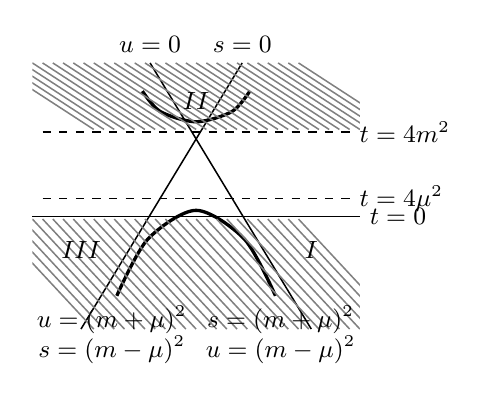
\begin{tikzpicture}[x=.65cm,y=.65cm,line width=.55pt,font=\small]
\draw (-3.2,0)--(3.2,0) node[right] {$t=0$};
\draw (-2.25,-2.2)--(.9,3.0) node[above] {$s=0$};
\draw (2.25,-2.2)--(-.9,3.0) node[above] {$u=0$};
\draw[dashed] (-3,1.65)--(3,1.65) node[right] {$t=4m^2$};
\draw[dashed] (-3,.35)--(3,.35) node[right] {$t=4\mu^2$};
\draw[very thick] plot[smooth] coordinates {(-1.05,2.45)(-.7,2.05)(0,1.85)(.7,2.05)(1.05,2.45)};
\draw[very thick] plot[smooth] coordinates {(-1.55,-1.55)(-.95,-.45)(0,.12)(.95,-.45)(1.55,-1.55)};
\begin{scope}\clip (-3.2,-2.3) rectangle (3.2,3.1);
\foreach \x in {-3,-2.8,...,3}{\draw[gray] (\x-1,3)--(\x+1,1.7);}
\foreach \x in {-3,-2.8,...,3}{\draw[gray] (\x-1,-.05)--(\x+1,-2.2);}
\end{scope}
\node at (0,2.25) {$II$}; \node at (-2.25,-.65) {$III$}; \node at (2.25,-.65) {$I$};
\node[below,align=center] at (-1.65,-1.55) {$u=(m+\mu)^2$\\$s=(m-\mu)^2$};
\node[below,align=center] at (1.65,-1.55) {$s=(m+\mu)^2$\\$u=(m-\mu)^2$};
\end{tikzpicture}

Fig.~6
\end{center}

If $\mu=0$ (particles 2 and 4 are photons), the lower branch of the hyperbola touches the axis $t=0$, and the physical regions are as shown in Fig.~7.

\SourcePage{294}{299}
If $m=\mu$, the boundaries (67.8) degenerate into the coordinate axes, and the physical regions are the three sectors shown in Fig.~8.

\begin{center}
\begin{minipage}{.47\linewidth}\centering
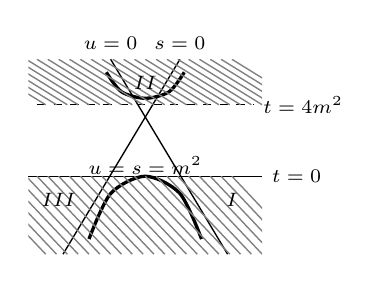
\begin{tikzpicture}[x=.55cm,y=.55cm,line width=.5pt,font=\scriptsize]
\draw (-2.7,0)--(2.7,0) node[right] {$t=0$};
\draw (-1.9,-1.8)--(.8,2.7) node[above] {$s=0$};
\draw (1.9,-1.8)--(-.8,2.7) node[above] {$u=0$};
\draw[dashed] (-2.5,1.65)--(2.5,1.65) node[right] {$t=4m^2$};
\draw[very thick] plot[smooth] coordinates {(-.9,2.4)(-.55,1.95)(0,1.8)(.55,1.95)(.9,2.4)};
\draw[very thick] plot[smooth] coordinates {(-1.3,-1.45)(-.8,-.4)(0,0)(.8,-.4)(1.3,-1.45)};
\begin{scope}\clip (-2.7,-1.8) rectangle (2.7,2.7);\foreach \x in {-3,-2.75,...,3}{\draw[gray] (\x-1,2.7)--(\x+.7,1.65);\draw[gray] (\x-1,0)--(\x+.7,-1.8);}\end{scope}
\node at (0,2.15) {$II$}; \node at (-2,-.55) {$III$}; \node at (2,-.55) {$I$};
\node at (0,.25) {$u=s=m^2$};
\end{tikzpicture}

Fig.~7
\end{minipage}\hfill
\begin{minipage}{.47\linewidth}\centering
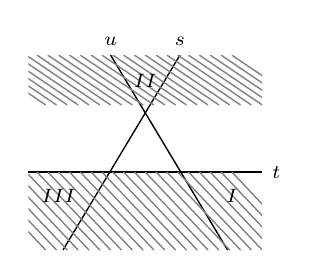
\begin{tikzpicture}[x=.55cm,y=.55cm,line width=.5pt,font=\scriptsize]
\draw (-2.7,0)--(2.7,0) node[right] {$t$};
\draw (-1.9,-1.8)--(.8,2.7) node[above] {$s$};
\draw (1.9,-1.8)--(-.8,2.7) node[above] {$u$};
\begin{scope}\clip (-2.7,-1.8) rectangle (2.7,2.7);\foreach \x in {-3,-2.75,...,3}{\draw[gray] (\x-1,2.7)--(\x+.7,1.55);\draw[gray] (\x-1,0)--(\x+.7,-1.8);}\end{scope}
\node at (0,2.1) {$II$}; \node at (-2,-.55) {$III$}; \node at (2,-.55) {$I$};
\end{tikzpicture}

Fig.~8
\end{minipage}
\end{center}

For four distinct masses, the equation
\begin{equation}
stu=as+bt+cu
\tag{67.10}
\end{equation}
defines a cubic curve whose branches bound the physical regions of the three channels, as in Fig.~9.

\begin{center}
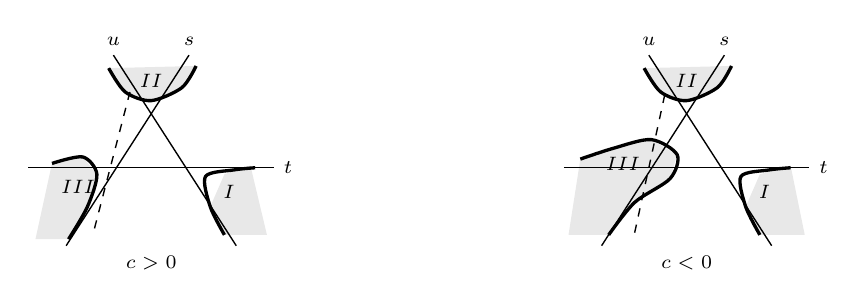
\begin{tikzpicture}[x=.6cm,y=.55cm,line width=.5pt,font=\scriptsize]
\begin{scope}[xshift=-3.4cm]
\fill[gray!18] (-.9,2.3)--(-.55,1.75)--(0,1.55)--(.65,1.85)--(.95,2.35)--cycle;
\fill[gray!18] (-2.1,.1)--(-1.45,.25)--(-1.15,-.15)--(-1.35,-.9)--(-1.75,-1.65)--(-2.45,-1.65)--cycle;
\fill[gray!18] (2.1,.05)--(1.55,-.15)--(1.25,-.9)--(1.55,-1.55)--(2.45,-1.55)--cycle;
\draw (-2.6,0)--(2.6,0) node[right] {$t$};\draw (-1.8,-1.8)--(.8,2.6) node[above] {$s$};\draw (1.8,-1.8)--(-.8,2.6) node[above] {$u$};
\draw[dashed] (-1.2,-1.4)--(-.45,1.75);
\draw[very thick] plot[smooth] coordinates {(-.9,2.3)(-.55,1.75)(0,1.55)(.65,1.85)(.95,2.35)};
\draw[very thick] plot[smooth] coordinates {(-2.1,.1)(-1.45,.25)(-1.15,-.15)(-1.35,-.9)(-1.75,-1.65)};
\draw[very thick] plot[smooth] coordinates {(1.55,-1.55)(1.25,-.9)(1.15,-.2)(1.75,-.05)(2.2,0)};
\node at (0,2) {$II$};\node at (-1.55,-.45) {$III$};\node at (1.65,-.55) {$I$};\node at (0,-2.2) {$c>0$};
\end{scope}
\begin{scope}[xshift=3.4cm]
\fill[gray!18] (-.9,2.3)--(-.55,1.75)--(0,1.55)--(.65,1.85)--(.95,2.35)--cycle;
\fill[gray!18] (-2.25,.2)--(-1.55,.45)--(-.75,.65)--(-.2,.3)--(-.35,-.25)--(-1.1,-.8)--(-1.65,-1.55)--(-2.5,-1.55)--cycle;
\fill[gray!18] (2.2,.05)--(1.55,-.15)--(1.25,-.9)--(1.55,-1.55)--(2.5,-1.55)--cycle;
\draw (-2.6,0)--(2.6,0) node[right] {$t$};\draw (-1.8,-1.8)--(.8,2.6) node[above] {$s$};\draw (1.8,-1.8)--(-.8,2.6) node[above] {$u$};
\draw[dashed] (-1.1,-1.5)--(-.45,1.75);
\draw[very thick] plot[smooth] coordinates {(-.9,2.3)(-.55,1.75)(0,1.55)(.65,1.85)(.95,2.35)};
\draw[very thick] plot[smooth] coordinates {(-2.25,.2)(-1.55,.45)(-.75,.65)(-.2,.3)(-.35,-.25)(-1.1,-.8)(-1.65,-1.55)};
\draw[very thick] plot[smooth] coordinates {(1.55,-1.55)(1.25,-.9)(1.15,-.2)(1.75,-.05)(2.2,0)};
\node at (0,2) {$II$};\node at (-1.35,.1) {$III$};\node at (1.65,-.55) {$I$};\node at (0,-2.2) {$c<0$};
\end{scope}
\end{tikzpicture}

Fig.~9
\end{center}

Let
\[
m_1\geqslant m_2\geqslant m_3\geqslant m_4.
\]
Then
\[
a\geqslant b\geqslant c,\qquad a>0,\qquad b>0.
\]
The curve (67.10) intersects the coordinate axes at points on the line
\[
as+bt+cu=0
\]
(the dashed lines in Fig.~9). Its form depends on the sign of $c$ as shown. For $c<0$, the physical region of the

\SourcePage{295}{300}
$u$-channel occupies part of the coordinate triangle; $s,t,u$ can then all be positive. The three coordinate axes are asymptotes of the corresponding branches. Conditions (67.2) generally add nothing to the boundaries fixed by (67.10): their equality lines do not cross the shaded physical regions, although some touch their boundaries at extreme values of $s,t,u$.

If one mass exceeds the sum of the other three, $m_1>m_2+m_3+m_4$, a fourth, decay channel is possible in addition to I, II, III:
\begin{equation}
\mathrm{IV}.\quad1\to\overline2+3+4.
\tag{67.11}
\end{equation}
In the rest frame of the decaying particle,
\[
q_1=(m_1,0),\quad q_2=(-\varepsilon_2,-\mathbf p_2),\quad q_3=(-\varepsilon_3,-\mathbf p_3),\quad q_4=(-\varepsilon_4,-\mathbf p_4),
\]
\[
\varepsilon_2+\varepsilon_3+\varepsilon_4=m_1,\qquad \mathbf p_2+\mathbf p_3+\mathbf p_4=0.
\]
The invariants are
\begin{equation}
\begin{aligned}
s&=m_1^2+m_2^2-2m_1\varepsilon_2,\\
t&=m_1^2+m_3^2-2m_1\varepsilon_3,\\
u&=m_1^2+m_4^2-2m_1\varepsilon_4.
\end{aligned}
\tag{67.12}
\end{equation}
Equation (67.1) now gives
\begin{equation}
\begin{aligned}
(m_3+m_4)^2&\leqslant s\leqslant(m_1-m_2)^2,\\
(m_2+m_4)^2&\leqslant t\leqslant(m_1-m_3)^2,\\
(m_2+m_3)^2&\leqslant u\leqslant(m_1-m_4)^2.
\end{aligned}
\tag{67.13}
\end{equation}
All three invariants are positive, so the physical region of the decay channel lies inside the coordinate triangle.

\ProblemHeading

1. Find the physical regions for three equal masses: $m_1\equiv m$, $m_2=m_3=m_4\equiv\mu$ (for example, $K+\pi\to\pi+\pi$).

\SolutionHeading Equation (67.10) becomes
\begin{equation}
stu=\mu^2(m^2-\mu^2)^2,
\tag{1}
\end{equation}
with
\[
s+t+u=3\mu^2+m^2.
\]

\SourcePage{296}{301}
Regions I, II, III are bounded by curves of identical form (for I, $s>0,t<0,u<0$, and similarly for II and III). If $m>3\mu$, (1) also has a branch, a closed curve with $s,t,u>0$, bounding the region of channel IV (Fig.~10).

\begin{center}
\begin{minipage}{.47\linewidth}\centering
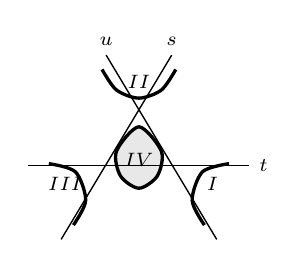
\begin{tikzpicture}[x=.52cm,y=.52cm,line width=.5pt,font=\scriptsize]
\fill[gray!18] plot[smooth cycle] coordinates {(-.55,.35)(0,.95)(.55,.35)(.45,-.25)(0,-.55)(-.45,-.25)};
\draw (-2.7,0)--(2.7,0) node[right] {$t$};\draw (-1.9,-1.8)--(.8,2.7) node[above] {$s$};\draw (1.9,-1.8)--(-.8,2.7) node[above] {$u$};
\draw[very thick] plot[smooth cycle] coordinates {(-.55,.35)(0,.95)(.55,.35)(.45,-.25)(0,-.55)(-.45,-.25)};
\draw[very thick] plot[smooth] coordinates {(-.9,2.35)(-.55,1.85)(0,1.65)(.55,1.85)(.9,2.35)};
\draw[very thick] plot[smooth] coordinates {(-2.2,.05)(-1.55,-.15)(-1.3,-.85)(-1.6,-1.45)};
\draw[very thick] plot[smooth] coordinates {(2.2,.05)(1.55,-.15)(1.3,-.85)(1.6,-1.45)};
\node at (0,2.05) {$II$};\node at (-1.8,-.45) {$III$};\node at (1.8,-.45) {$I$};\node at (0,.15) {$IV$};
\end{tikzpicture}

Fig.~10
\end{minipage}\hfill
\begin{minipage}{.47\linewidth}\centering
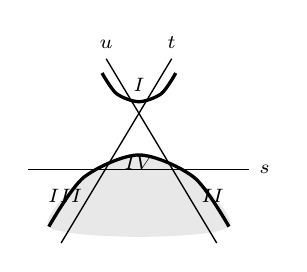
\begin{tikzpicture}[x=.52cm,y=.52cm,line width=.5pt,font=\scriptsize]
\fill[gray!18] plot[smooth cycle] coordinates {(-2.2,-1.4)(-1.35,-.2)(0,.35)(1.35,-.2)(2.2,-1.4)(0,-1.65)};
\draw (-2.7,0)--(2.7,0) node[right] {$s$};\draw (-1.9,-1.8)--(.8,2.7) node[above] {$t$};\draw (1.9,-1.8)--(-.8,2.7) node[above] {$u$};
\draw[very thick] plot[smooth] coordinates {(-.9,2.35)(-.55,1.85)(0,1.65)(.55,1.85)(.9,2.35)};
\draw[very thick] plot[smooth] coordinates {(-2.2,-1.4)(-1.35,-.2)(0,.35)(1.35,-.2)(2.2,-1.4)};
\node at (0,2.05) {$I$};\node at (-1.8,-.65) {$III$};\node at (1.8,-.65) {$II$};\node at (0,.15) {$IV$};
\end{tikzpicture}

Fig.~11
\end{minipage}
\end{center}

2. Find the same regions for $m_1\equiv m$, $m_2\equiv\mu$, $m_3=m_4=0$, $m>\mu$ (for example, $\mu+\nu\to e+\nu$).

\SolutionHeading Condition (67.5) becomes
\[
stu\geqslant m^2\mu^2s,
\]
with $s+t+u=m^2+\mu^2$. The physical regions are bounded by the axis $s=0$ and the two branches of $tu=m^2\mu^2$ (Fig.~11).

3. Find the same regions for $m_1=m_3\equiv m$, $m_2=0$, $m_4=\mu$, with $m>2\mu$ (for example, $\rho+\gamma\to\rho+\pi^0$).

\SolutionHeading The boundary equation (67.10) becomes
\[
stu=a(s+u)+bt,\qquad ah=m^2\mu^4,
\]
\[
bh=m^4(2m^2-\mu^2),\qquad h=2m^2+\mu^2.
\]
Eliminating $u$ gives
\[
t^2+\left(\frac{b-a}{s}+s-h\right)t+\frac{ah}{s}=0.
\]
At fixed $s$ this is a quadratic in $t$. For $s>(m+\mu)^2$ (the $s$-channel region), each $s$ has two negative values of $t$. At $s=(m+\mu)^2$ the roots merge at $t=-m\mu^2/(m+\mu)$. The $s$-channel boundary is shown in Fig.~12. Its lower branch approaches $u=0$ asymptotically, and the upper branch crosses this axis at $t=\mu^4/(\mu^2-m^2)$.

\begin{center}
\begin{tikzpicture}[x=.65cm,y=.55cm,line width=.55pt,font=\scriptsize]
\fill[gray!18] plot[smooth] coordinates {(-1.15,2.65)(-.7,2.25)(0,2.05)(.7,2.25)(1.15,2.65)} -- cycle;
\fill[gray!18] (-3.4,0)--(-3.2,-.2)--(-2.0,-.35)--(-.75,-1.05)--(0,-1.15)--(-2.65,-2.2)--cycle;
\fill[gray!18] (3.4,0)--(3.2,-.2)--(2.0,-.35)--(.75,-1.05)--(0,-1.15)--(2.65,-2.2)--cycle;
\draw (-3.8,0)--(3.8,0) node[right] {$t$};\draw (-2.65,-2.2)--(1.15,3.0) node[above] {$s$};\draw (2.65,-2.2)--(-1.15,3.0) node[above] {$u$};
\draw[dashed] (-3.4,2)--(3.4,2) node[right] {$t=4m^2$};
\draw[dashed] (-2.7,-1.15)--(2.7,-1.15) node[right] {$t=-\dfrac{m\mu^2}{m+\mu}$};
\draw[very thick] plot[smooth] coordinates {(-1.15,2.65)(-.7,2.25)(0,2.05)(.7,2.25)(1.15,2.65)};
\draw[very thick] plot[smooth] coordinates {(-3.2,-.2)(-2.0,-.35)(-.75,-1.05)(0,-1.15)};
\draw[very thick] plot[smooth] coordinates {(0,-1.15)(.75,-1.05)(2.0,-.35)(3.2,-.2)};
\node at (0,2.45) {$t$};\node at (-2.6,-.55) {$u$};\node at (2.6,-.55) {$s$};
\end{tikzpicture}

Fig.~12
\end{center}

The $u$-channel region is symmetric to the $s$-channel region, while the $t$-channel region is positioned as shown.
